% 封面
\begin{frame}
  \titlepage
\end{frame}


% 目录
\begin{frame}{Content}
  \tableofcontents
\end{frame}


% 在开头与每个小节导入带强调的目录, 需要编译两遍!
% 目录以 Section &  Subsection 指出
% \AtBeginSection[]
% {
%   \begin{frame}
%     \frametitle{Table of Contents}
%     \tableofcontents[currentsection]
%   \end{frame}
% }


% 先验知识
\section{Prerequsite knowledge}
\subsection{GARCH Family Models}
\begin{frame}{GARCH Model}
  \begin{block}{GARCH ($p,q$) \cite{bollerslev1986_garch}}
    Series $\left\{a_{t}\right\}$ follows a GARCH ($p,q$) model if
    \begin{displaymath}
			\begin{array}{c}
				a_{t}=\sigma_{t | t-1}\varepsilon_{t},\\
				\sigma_{t | t-1}^2 = \omega+\sum_{i=1}^q{\alpha_{i}a_{t-i}^2} + \sum_{j=1}^p{\beta_{j}\sigma_{t-j | t-j-1}^2},  
			\end{array}
		\end{displaymath}
		where $\{a_{t}\}$ is a zero mean time series, $\omega > 0$, $\alpha_{i} \geq 0$, $\beta_{j} \geq 0$ for $i>0$, $j>0$. ${\left\{\varepsilon_{t}\right\}}$ is a sequence of i.i.d. random variables with mean zero and variance one.
  \end{block}
  \begin{itemize}
    \item Note that p is the order of GARCH part, q is the order of ARCH part.
    \item GARCH($p, q$) for $a_{t}$ implies \red{ARMA($\max(p,q)$, $p$)} for $a_{t}^2$.
    \item \red{$\sum_{i=1}^{q}\alpha_{i}+\sum_{i=1}^{p}\beta_{i}<1$}, under the assumption of finite variance. 
  \end{itemize}
\end{frame}

\begin{frame}{GARCH Model Cont' d}
  \small{
  \begin{block}{IGARCH($1,1$) \cite{engle1986_igarch}}
    Series $\left\{a_{t}\right\}$ follows an integrated GARCH($1,1$) model if
    \begin{displaymath}
      \begin{array}{c} % 两行的公式用array环境!
        a_{t}=\sigma_{t \mid t-1} \varepsilon_{t}, \\
        \sigma_{t \mid t-1}^{2}=\alpha_{0}+\beta_{1}\sigma_{t-1 \mid t-2}^2+\red{(1-\beta_{1})}a_{t-1}^{2}
      \end{array}
    \end{displaymath}
    The unconditional variance of $a_{t}$ is not defined.
  \end{block}
  
  \begin{block}{TGARCH$(p,q)$ \cite{zakoian1994_tgarch}}
    Series $\left\{a_{t}\right\}$ follows an threshold GARCH ($p,q$) model if
    \begin{displaymath}
      \begin{array}{c}
        \sigma_{t \mid t-1}^{2}=\alpha_{0}+\sum_{i=1}^{q}\left(\alpha_{i}\red{+\gamma_{i} N_{t-i}}\right) a_{t-i}^{2}+\sum_{j=1}^{p} \beta_{j} \sigma_{t-j \mid t-j-1}^{2},\\
        N_{t-i}=\left\{\begin{array}{ll}
          1 & \text { if } a_{t-i}<0 \\
          0 & \text { if } a_{t-i} \geq 0
          \end{array}\right.
      \end{array}
    \end{displaymath}
    From the model, a positive $a_{t-i}$ contributes $\alpha_{i}a_{t-i}^2$ to $\sigma_{t \mid t-1}^2$, whereas a negative $a_{t-i}$ has a larger impact $(\alpha_{i}+\gamma_{i})a_{t-i}^2$ with $\gamma_{i}>0$.
  \end{block}}
\end{frame}

\begin{frame}{ARMA-GARCH model}
  \begin{block}{ARMA(p,q) Model}
    \begin{displaymath}
      r_{t} =  \phi_{0}+\sum_{i=1}^{p} \phi_{i} r_{t-i}+\varepsilon_{t}-\sum_{i=1}^{q} \theta_{i} \varepsilon_{t-i}
    \end{displaymath}
    where ${\varepsilon_{t}}$ is a white noise series and p and q are non-negative integers.
  \end{block}

  \begin{block}{ARMA(p,q)-GARCH(m,n) model}
    \begin{displaymath}
      \begin{array}{c}
        r_{t} =  C +\underbrace{\sum_{i=1}^{p} \phi_{i} r_{t-i}+\varepsilon_{t}-\sum_{i=1}^{q} \theta_{i} \varepsilon_{t-i}}_{\textrm{ARMA part}} + \underbrace{\sigma_{t \mid t-1}\varepsilon_{t}}_{\textrm{GARCH part}},\\ 
        % a_{t}=\sigma_{t \mid t-1}\varepsilon_{t},\\
          \\
        \sigma_{t \mid t-1}^2 = \omega + \sum_{j=1}^m{\beta_{j}\sigma_{t-j \mid t-j-1}^2} + \sum_{i=1}^n{\alpha_{i}a_{t-i}^2}
      \end{array}
    \end{displaymath}
  \end{block}
\end{frame}


% 背景与目标
\section{Background and Object}
\begin{frame}{Research background}
  \begin{itemize}
    \item For certain \nb{stocks}:
      \begin{itemize}
        \item the \red{expected revenue} is measured by the conditional expectation of the return rate $E(r_{t}\mid F_{t-1})$,
        \item the \red{risk size} is measured by the conditional variance of the return rate $Var(r_{t}\mid F_{t-1})$.
        % \item the conditional variance is not constant because of volatility clustering.
      \end{itemize}
    \item The \nb{ARMA-GARCH models} 
      \begin{itemize}
        \item \red{sketch the conditional mean and conditional variance} of time series simultaneously and
        \item have good interpretability and extensibility.
      \end{itemize}
    \item Two \nb{problems} hinder the application of ARMA-GARCH models in the Chinese stock market:
      \begin{itemize}
        \item more evidence on the validity of \red{ARMA-GARCH model extensions} (later introduced) for the Chinese stock market needs to be collected,
        \item the \red{model establishment process} is unreasonable .
      \end{itemize}
  \end{itemize}
\end{frame}

\begin{frame}{Research object}
  In this study we compare:
  \begin{itemize}
    \item the \nb{ARMA-GARCH model extensions}, including: 
      \begin{itemize}
        \item \red{GARCH family models} like: GARCH, IGARCH, TGARCH,
        \item \red{Heavy-tailed innovation distributions} like: Normal distribution, Student's t distribution, Generalized error distribution and their skewed extensions,
      \end{itemize}
    \item two \nb{model establishment methods}, including: 
      \begin{itemize}
        \item the \red{Tsay's method} \cite{tsay2005_financial_time_series}: determines the order of the ARMA-GARCH model \red{sequentially} then estimates the parameters \red{jointly},
        \item the \red{All possible regression method}: directly estimates \red{all} the models within the search scope and selects the best model with the lowest AIC.
      \end{itemize}
  \end{itemize}
\end{frame}

\begin{frame}{Abbreviation}
  To save space, in this paper we use the following abbreviations:

  \begin{table}[htbp]
    \begin{tabular}{@{\hspace*{2.8em}}rl}
    SSEC & is the Shanghai Stock Exchange Composite Index, \\
    SZI & is the Shenzhen Component Index, \\
    N   & is the Normal distribution, \\
    T   & is the Student's t distribution, \\
    GED & is the Generalized error distribution, \\
    SN  & is the skewed Normal distribution, \\
    ST  & is the skewed Student's t distribution, \\
    SGED & is the skewed Generalized error distribution. \\
    \end{tabular}
  \end{table}
\end{frame}

  
  
\section{Empirical study}
\subsection{Dataset}
\begin{frame}{Dataset}
  \vspace{-10pt}
  \begin{figure}[htbp]
    \centering
    \caption{Closing price series of SSEC and SZI and selected time spans}
    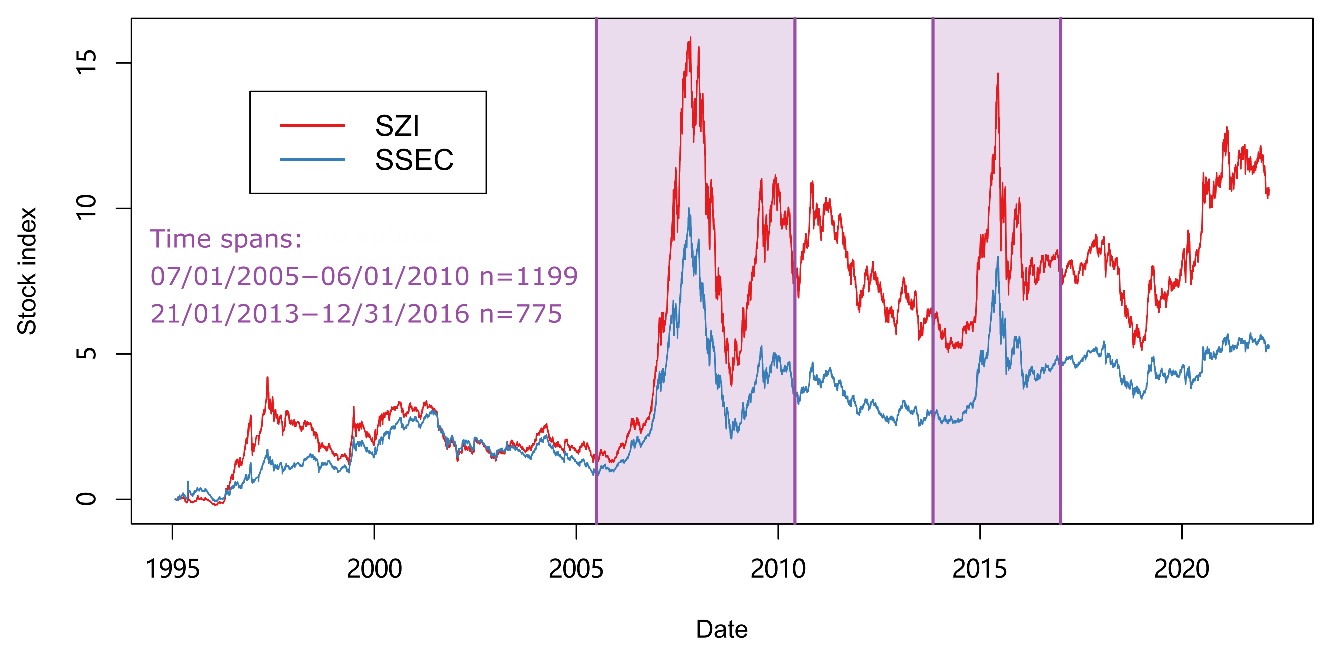
\includegraphics[width = 1\columnwidth]{fig/Closed index series of SSEC and SZI_trimed_modified.eps}
    \label{fig: Closed index series of SSEC and SZI and selected time spans}
  \end{figure}

  \vspace{-20pt}
  Time spans contain the \red{bull, bear and consolidation} period are chosen to capture the complete dynamic.
\end{frame}

\begin{frame}
  \vspace{-5pt}
  \begin{figure}[htbp]
    \centering
    \caption{Exploration data analysis on one dataset}
    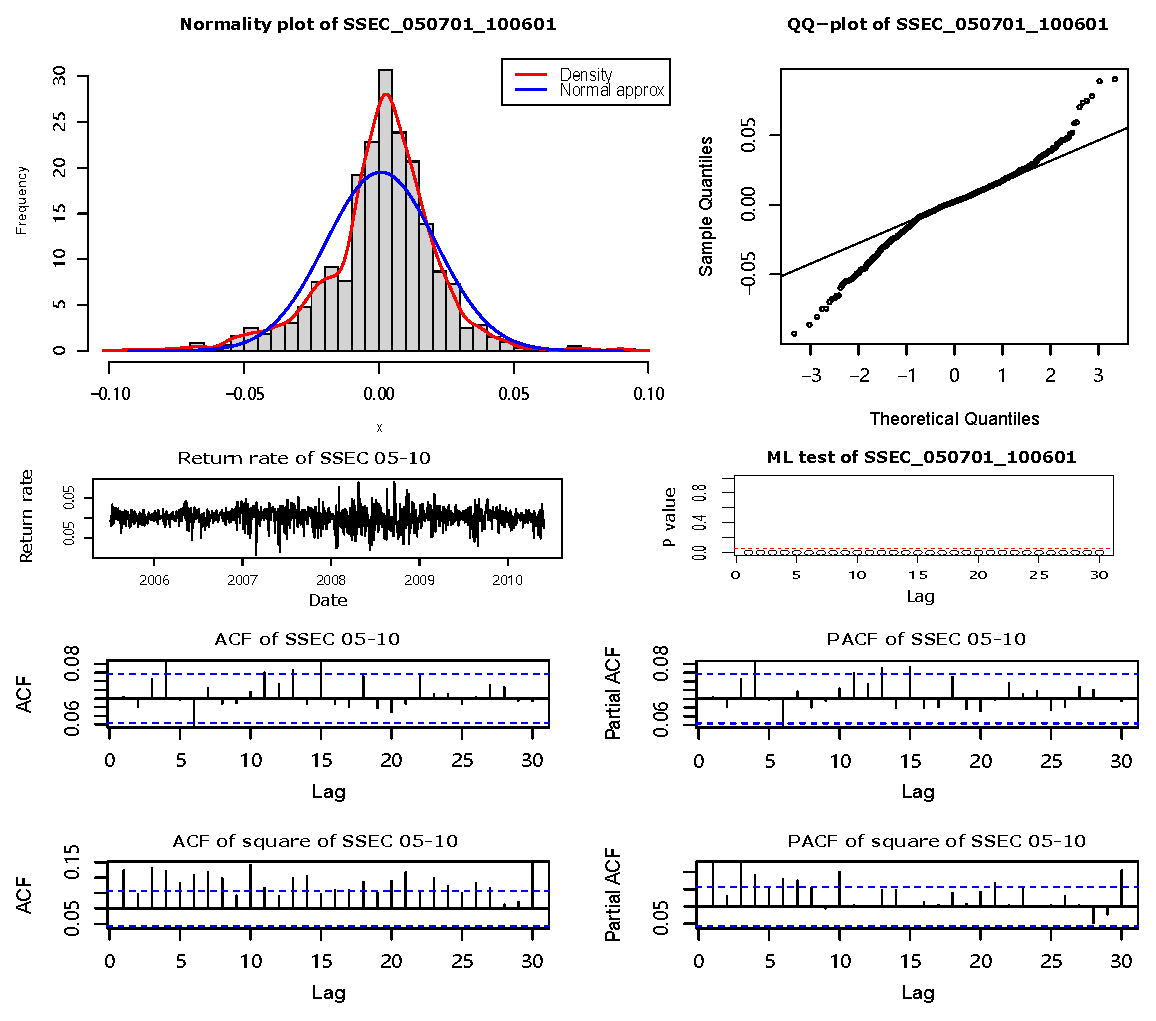
\includegraphics[width = .75\columnwidth]{fig/combine.eps}
    \label{fig: Exploration data analysis on one dataset}
  \end{figure}
\end{frame}


\subsection{Research scheme}
\begin{frame}{Research scheme}
  \begin{table}[htbp]
    \vspace{-20pt}
    % \setlength\tabcolsep{3pt}
    % \renewcommand\arraystretch{.5}
    \centering
    \caption{Scopes of the model establishment for different schemes}
    \resizebox{.8\textwidth}{!}{
      \begin{tabular}{cclcll}
        \toprule[2pt]
        \multirow{2}[2]{*}{Scheme} & \multirow{2}[2]{*}{ARMA} & \multicolumn{2}{c}{Conditional Var model} & \multicolumn{1}{c}{\multirow{2}[2]{*}{Innov. dist.}} & \multicolumn{1}{c}{\multirow{2}[2]{*}{Model selection method}} \\
    
        \cmidrule(lr){3-4}       
         &     & \multicolumn{1}{c}{Model} & Scope & \multicolumn{1}{c}{} &  \\
    
        \cmidrule(lr){1-6}
        1   & (0,0)-(4,4) & GARCH & (0,0)-(3,3) & N   & Tsay's method \\
    
        2   & (0,0)-(4,4) & GARCH & (0,0)-(3,3) & N   & All possible regression \\
    
        3   & (0,0)-(4,4) & GARCH & (0,0)-(3,3) & N   & All possible regression \\
        & & TGARCH & & & \\
        & & IGARCH & & & \\
    
        4   & (0,0)-(4,4) & GARCH & (0,0)-(3,3) & N, T, GED & All possible regression \\
        & & TGARCH & & & \\
        & & IGARCH & & & \\
    
        5   & (0,0)-(4,4) & GARCH & (0,0)-(3,3) & N, T, GED, & All possible regression \\
        & & TGARCH & & SN, ST, SGED & \\
        & & IGARCH & & & \\
    
        \bottomrule[2pt]
      \end{tabular}
    }
    \label{tab:Scope of model establishment for different methods}
  \end{table}
  
  \begin{itemize}
    % \item Scheme 1 and 2: compare the credibility of two model establishment methods.
    \item Scheme 3 and 4, provide the \red{local best models} rest on the Normal and non-skewed assumption respectively. Thus we can find the right balance between model complexity and computational efficiency for the All possible regression method.
    % \item Scheme 3: checks the validity of IGARCH models and TGARCH models.
    % \item Scheme 4: study the capability of the Normal, Student's t and GED innovation distributions.
    % \item Scheme 5: compared the corresponding skewed derivatives.
  \end{itemize}
\end{frame}


\subsection{Estimation result}
\begin{frame}{Estimation result}
  \begin{table}[htbp]
    \vspace{-10pt}
    \setlength\tabcolsep{2pt}
    \renewcommand\arraystretch{.6}
    \centering
    \caption{The best models and corresponding AIC}
    \vspace{-10pt}
    \resizebox{\textwidth}{!}{
      \begin{threeparttable}
        \begin{tabular}{ccccclrccclr}
          \toprule[2pt]
          \multirow{2}[2]{*}{Dataset} & \multirow{2}[2]{*}{Scheme} &\multicolumn{5}{c}{05-10} & \multicolumn{5}{c}{13-16} \\

          \cmidrule(lr){3-7} \cmidrule(lr){8-12} 
          & & ARMA-GARCH & $\mu$ & $\omega$ & \multicolumn{1}{c}{Innov. Dist.} & \multicolumn{1}{c}{AIC} & ARMA-GARCH & $\mu$ & $\omega$ & \multicolumn{1}{c}{Innov. Dist.} & \multicolumn{1}{c}{AIC} \\

          \cmidrule(lr){1-7} \cmidrule(lr){8-12} 
          \multicolumn{1}{c}{\multirow{5}[2]{*}{SSEC}} & 1   & (2,2)-(1,1) & 0   & 0   & N   & \gre{-5.109} & (3,3)-(1,1) & 0   & 0   & N   & \gre{-5.736} \\
              & 2   & (4,4)-(1,1) & 0   & 0   & N   & \gre{-5.112}      & (3,3)-(1,1) & 0   & 0   & N   & \gre{-5.736} \\
              & 3   & (2,2)-I(1,1) & 0   & 0   & N   & \textcolor{red}{-5.113}     & (5,4)-I(1,1) & 0   & 0   & N   & \textcolor{red}{-5.746} \\
              & 4   & (4,3)-I(1,1) &     & 0   & GED & \textcolor{red}{-5.192}     & (3,3)-I(1,1) &     & 0   & GED & \textcolor{red}{-5.847} \\
              & 5   & (4,3)-I(1,1) & 0   & 0   & SGED & -5.205     & (3,3)-I(1,1) & 0   & 0   & SGED & -5.847 \\

          \cmidrule(lr){1-7} \cmidrule(lr){8-12} 
          \multicolumn{1}{c}{\multirow{5}[2]{*}{SZI}} & 1   & (2,2)-(1,1) & 0   & 0   & N   & \gre{-4.891} & (3,3)-(1,1) & 0   & 0   & N   & \gre{-5.346} \\
              & 2   & (4,3)-(1,1) & 0   & 0   & N   & \gre{-4.894}     & (2,2)-(1,1) & 0   & 0   & N   & \gre{-5.353} \\
              & 3   & (4,3)-I(1,1) & 0   & 0   & N   & \textcolor{red}{-4.898}     & (2,2)-I(1,1) & 0   & 0   & N   & \textcolor{red}{-5.357} \\
              & 4   & (1,1)-I(1,1) & 0   & 0   & GED & \textcolor{red}{-4.949}     & (2,2)-I(1,1) & 0   & 0   & GED & \textcolor{red}{-5.456} \\
              & 5   & (3,3)-I(1,1) & 0   & 0   & SGED & -4.964     & (2,2)-I(1,1) & 0   & 0   & SGED & -5.466 \\
          \bottomrule[2pt]
          \end{tabular}
    \begin{tablenotes}
      \item [a] I stands for the IGARCH model.
    \end{tablenotes}
    \end{threeparttable}
    }
    \label{tab:The best model of the five establishment schemes for four datasets}
  \end{table}

  \vspace{-10pt}
  
  \begin{itemize}
    \footnotesize
    \item The \red{All possible regression method} shows better performance in the ARMA-GARCH model establishment.
    \item For the conditional variance model, the \red{IGARCH (1,1)} is recommended.
    \item For heavy-tailed innovation distributions, the \red{GED} and \red{SGED} are recommended based on non-skewed and skewed innovation distribution assumptions respectively.
  \end{itemize}
\end{frame}


% 分两列,一列图,一列文字
\subsection{Residual and prediction}
\begin{frame}{Residual analysis}
  \begin{columns} % 分列
    \column{0.5\textwidth} % 文字列,0.x 倍宽
    \begin{figure}[htbp]
      \centering
      \caption{QQ-plots of five schemes on dataset SSEC 05-10}
      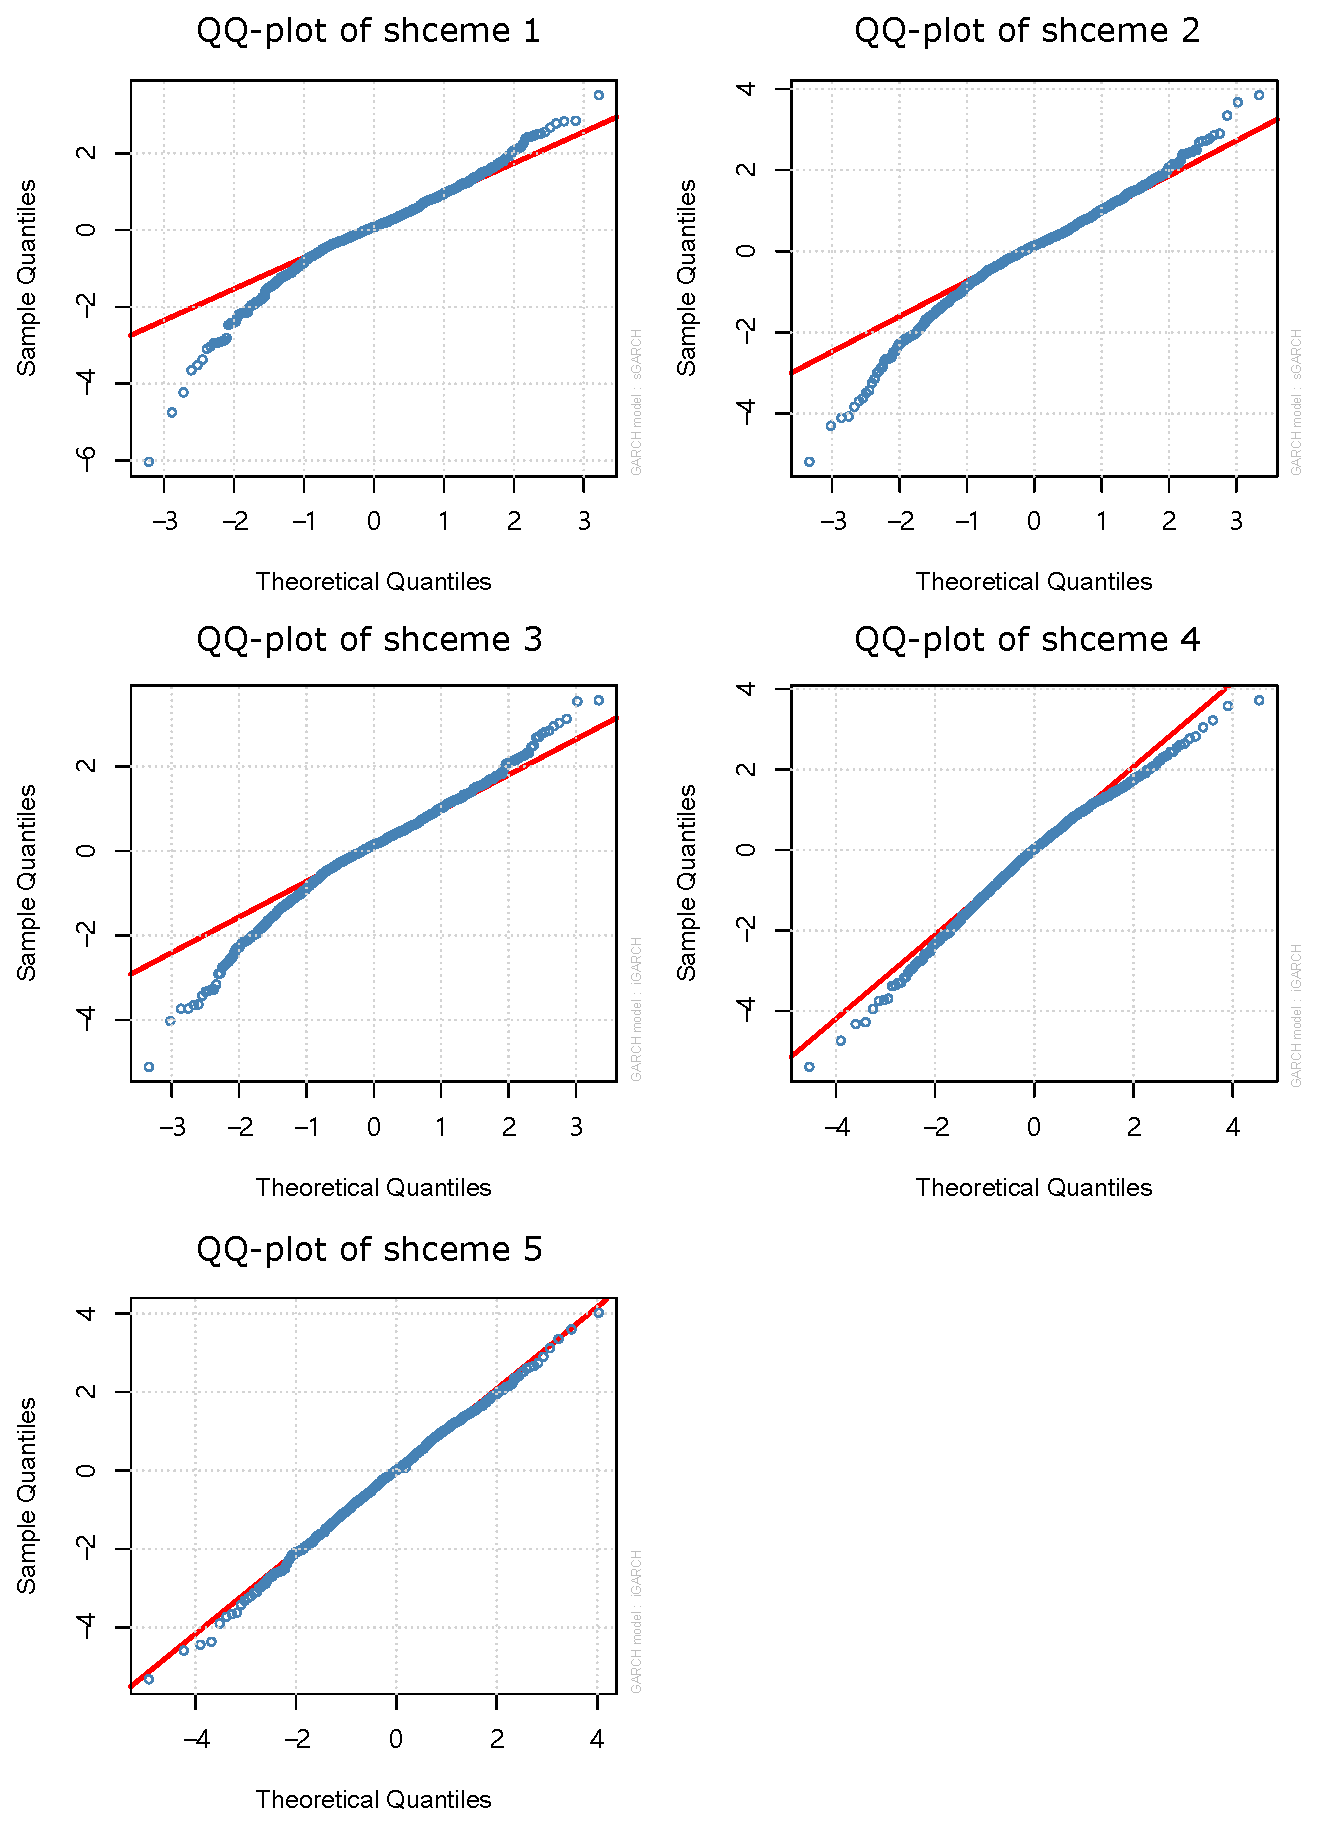
\includegraphics[width = .76\columnwidth]{fig/ssec0510_pred_qqplot_agg_colored.eps}
      \label{fig:QQ-plot of five schemes for dataset SSEC 05-10}
    \end{figure}
    
    \column{0.5\textwidth}
    From the BDS-test, residuals are independent under 95\% of confidence level for all schemes.
    \begin{itemize}
      % \item From the BDS-test, residuals are independent under 95\% of confidence level for all schemes.
      \item Scheme 1, 2 and 3 [Normal]: scatter points \red{deviate} from qq-lines on both sides, especially on the left-hand side.
      \item Scheme 4 [GED]: the scatter points converge towards the qq-lines but shows a \red{left bias}.
      \item Scheme 5 [SGED]: the scatter points fit the qq-lines quite well even for outliers.
    \end{itemize}

  \end{columns}
\end{frame}
  
\begin{frame}{Prediction}
  \vspace{-20pt}
  \begin{columns} % 分列
    \column{0.54\textwidth}{ % 文字列,0.x 倍宽
    \begin{figure}[htbp]
      \centering
      \caption{ten-days ahead predictions and corresponding confidence intervals}
      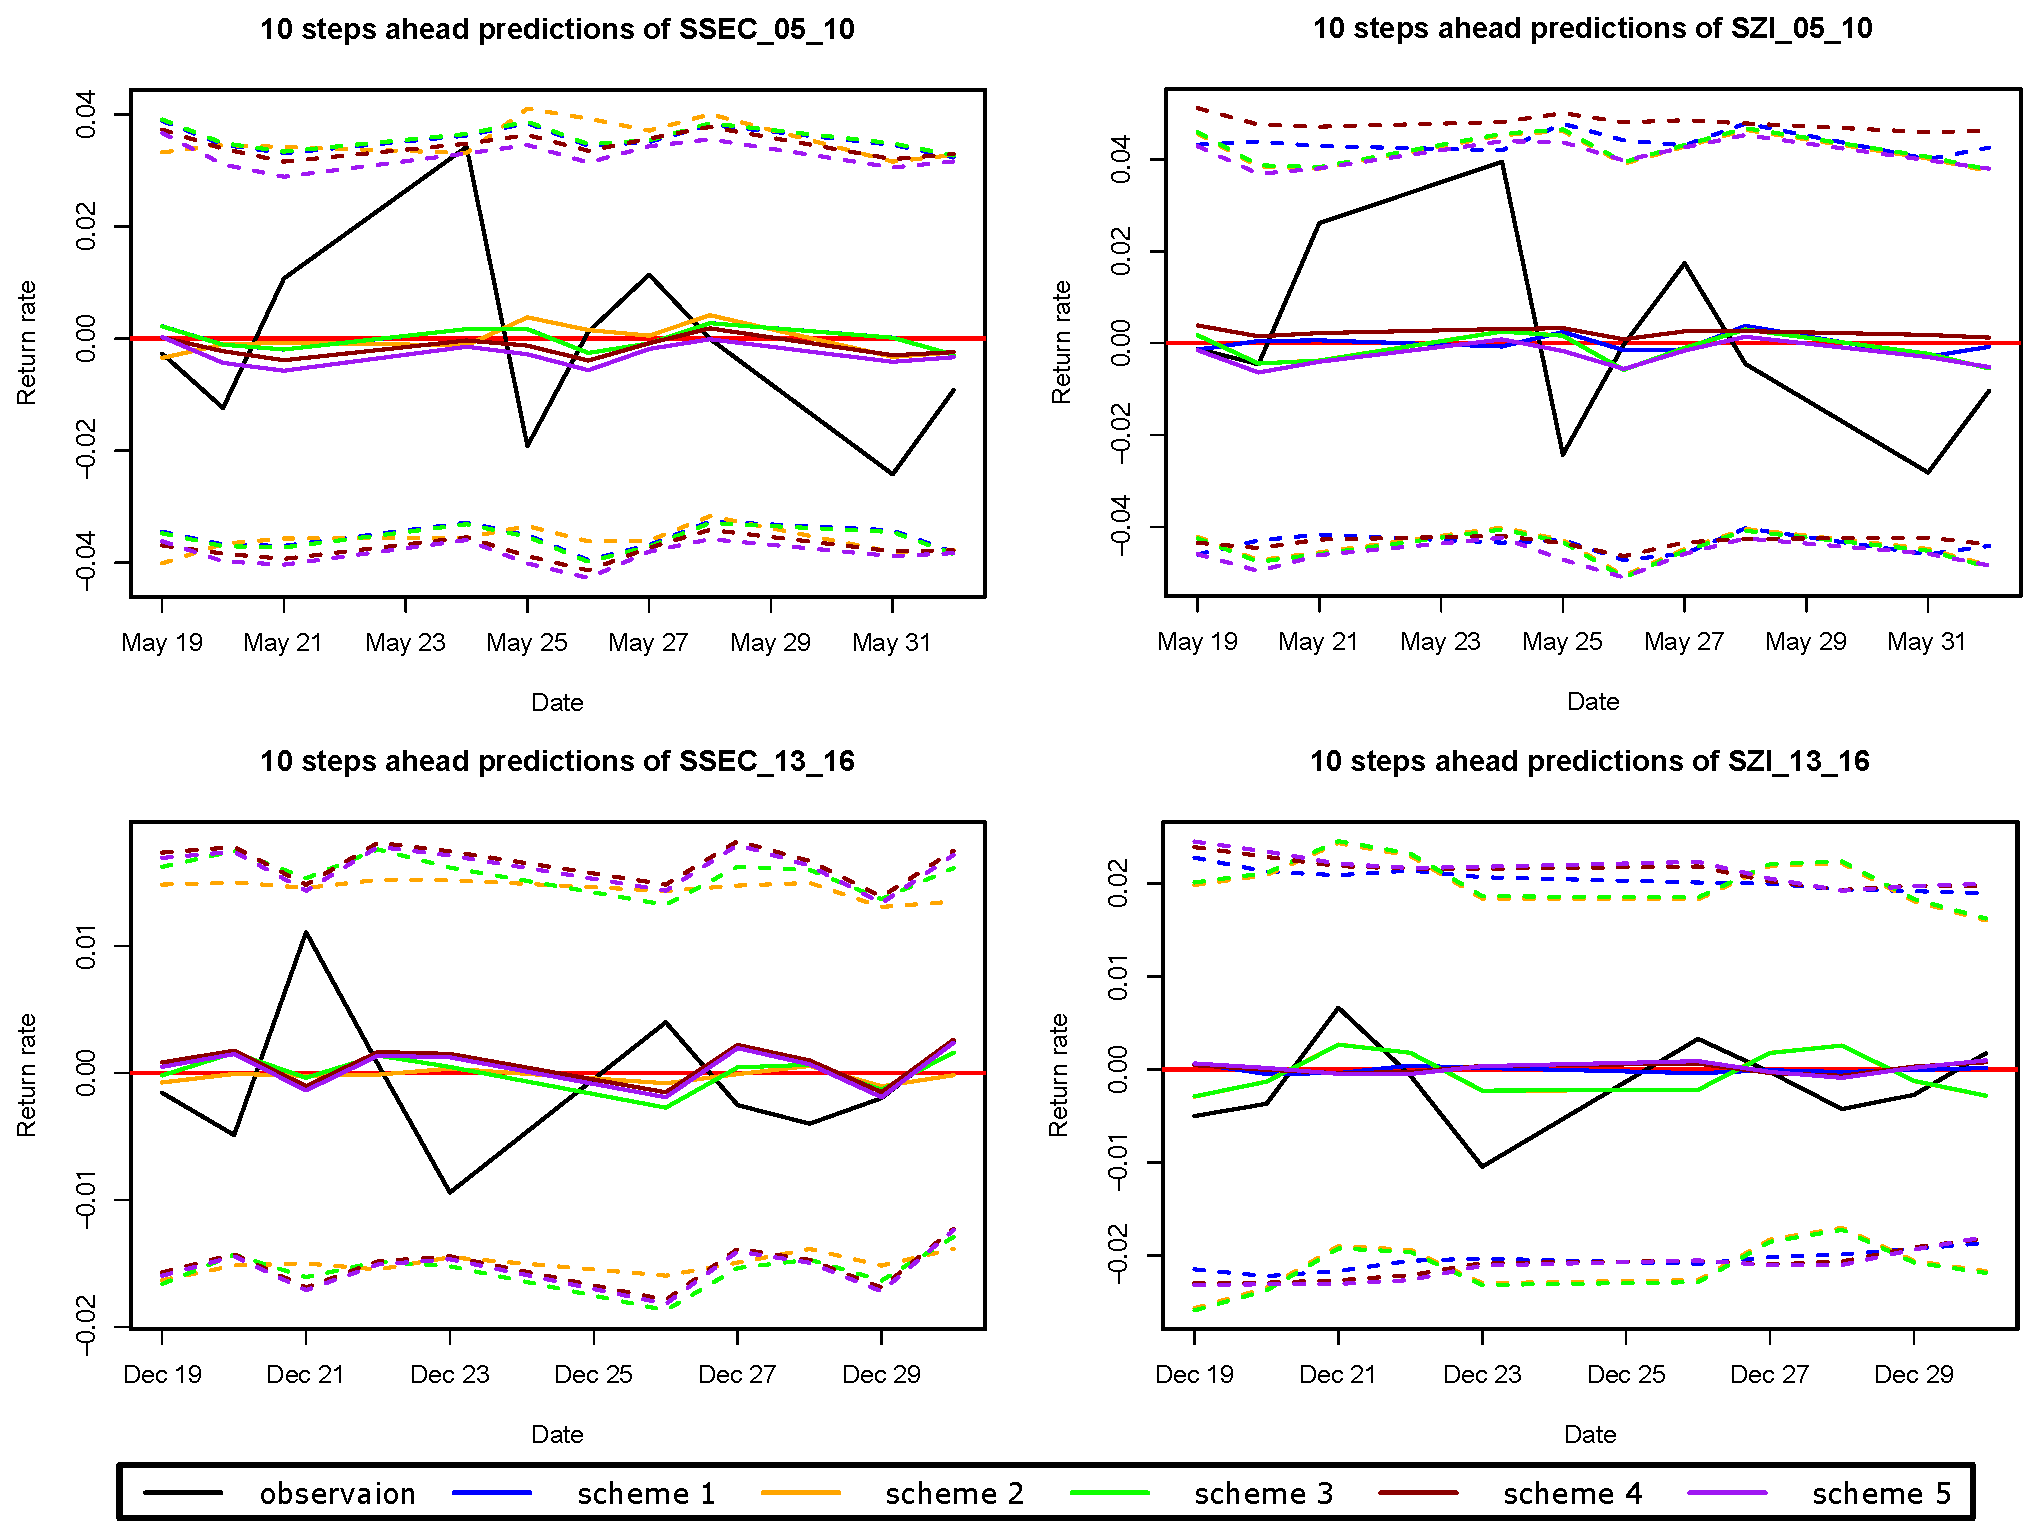
\includegraphics[width = .9\columnwidth]{fig/pred_plot_agg.eps}
      \label{fig:10 step ahead forecasting value and confidence interval}
    \end{figure}
    }

    \column{0.46\textwidth}{
    \begin{table}
      \centering
      \caption{Loss functions ($\times$1000) of predictions}
      \vspace{-10pt}
      \resizebox{\textwidth}{!}{
        \begin{tabular}{lrrrrr}
          \toprule[2pt]
          & \multicolumn{1}{c}{Scheme 1} & \multicolumn{1}{c}{Scheme 2} & \multicolumn{1}{c}{Scheme 3} & \multicolumn{1}{c}{Scheme 4} & \multicolumn{1}{c}{Scheme 5} \\
          \cmidrule(lr){1-6}
    
          & \multicolumn{5}{c}{SSEC 05-10} \\
          \cmidrule(lr){1-6}
  
          MSE & \gre{0.261}  & \gre{0.260}  & 0.261  & 0.253  & \textcolor{red}{0.252} \\
          MAE & 13.188 & 12.517 & 13.184 & 12.742 & 12.184 \\
          \cmidrule(lr){1-6}
    
          & \multicolumn{5}{c}{SZI 05-10} \\
          \cmidrule(lr){1-6}
    
          MSE & \gre{0.416} & \gre{0.406} & 0.406 & 0.410 & \textcolor{red}{0.400} \\
          MAE & 16.076 & 15.808 & 15.805 & 15.580 & 15.409 \\
          \cmidrule(lr){1-6}
          
          & \multicolumn{5}{c}{SSEC 13-16} \\		\cmidrule(lr){1-6}
    
          MSE & \gre{0.030} & \textcolor{red}{0.030} & 0.035 & 0.039 & 0.039 \\
          MAE & 4.282 & 4.282 & 4.567 & 4.889 & 4.737 \\
          \cmidrule(lr){1-6}
          
          & \multicolumn{5}{c}{SZI 13-16} \\
          \cmidrule(lr){1-6}
    
          MSE & \gre{0.024} & \textcolor{red}{0.020} & 0.020 & 0.024 & 0.024 \\
          MAE & 3.967 & 3.943 & 3.949 & 3.769 & 3.700 \\
          \bottomrule[2pt]
        \end{tabular}
      }
        \label{tab:Loss functions of the predictions}
    \end{table}
    }
  \end{columns}

  \begin{itemize}
    \footnotesize
    \item Scheme 1 with 2: the best models of the \red{All possible regression method} yield better prediction performance in three datasets.
    \item Scheme 2-5, the \red{IGARCH-SGED} achieves less loss in time span 05-10 but the \red{GARCH-Normal} are better in time span 13-16.
    
    Because the sample size in time span 13-16 (775) is much less than that of time span 05-10 (1199).
  \end{itemize}
\end{frame}


\section{Discussion and conclusion}
\subsection{Discussion}
\begin{frame}{Discussion}
  \begin{table}[htbp]
    \centering
    \caption{Comparison of two model selection methods}
    \resizebox{\textwidth}{!}{
      \begin{tabular}{p{12em}p{13em}p{15em}}
      \toprule[2pt]
      \multicolumn{1}{c}{} & Tsay's method & All possible regression method \\

      \cmidrule(lr){1-3}
      Computational requirement & Low & High \\

      Expansibility & Only applicable to determine the orders of certain ARMA-GARCH models & Applicable for different GARCH models and innovation distributions \\

      Model establishing procedure & Determine the orders of ARMA and GARCH sequentially & Determine the orders of ARMA and GARCH simutaneously \\
      
      User requirement & Specify orders from the EACF plots twice at least & No statistical discrimination required from the user \\

      Object & Find a significant model but the optimality isn't checked & Report the significant model outperforming other models under AIC \\
      \bottomrule[2pt]
      \end{tabular}
    }
    \label{tab:Comparison of two model selection methods}
  \end{table}
\end{frame}


\subsection{Conclusion}
\begin{frame}{Conclusion}
  Conclusion:
  \begin{itemize}
    \item The \red{All possible regression method} is recommended.
    \item The \red{IGARCH (1,1)} model is recommended to be the conditional variance model to eliminate the computational intensity.
    \item The \red{Generalized error distribution} and \red{skewed Generalized error distribution} are suitable for large datasets (\red{n>1000} in our case) under non-skewed and skewed assumption respectively.
    \item The \red{GARCH (1,1) }model and \red{Normal distribution} is preferred for small datasets (\red{n<1000} in our case) to avoid overfitting.
    \item The choice of the searching scope of the All possible regression method can follow the rules above to simplify computation.
  \end{itemize}

  Further study:
  \begin{itemize}
    \item To capture the leverage property, TGARCH models should be built for different market states individually.
    \item For the All possible regression method, \red{new criteria} are needed to moderate overfitting in small datasets.
  \end{itemize}
\end{frame}

% \begin{frame}{Further study}
%   \begin{itemize}
%     \item The TGARCH model is not significant for all four datasets. To capture the leverage property, the time span should be trimed to include only one market status.
%     \item A detailed investigation of the likelihood function of ARMA-GARCH models under different innovation distributions should to be carried out.
%   \end{itemize}
% \end{frame}


%--------- THANK YOU Text --------------------------
% \begin{frame}
%   \centering
%   \begin{block}
%     \scshape
%       \begin{center}
%         \large\emph{Thank You For Your Precious Feedback And Constructive Criticism!}
%       \end{center}
%   \end{block}
% \end{frame}
%----------------------------------------------------


%----------- REFERENCES  -------------
%----------- No editing in references section ----------
%----------- edit only in References.bib ----------
	\begin{frame}[allowframebreaks]{References}
		\bibliography{section/references}
	\end{frame}